\documentclass[conference]{IEEEtran}
\IEEEoverridecommandlockouts
% The preceding line is only needed to identify funding in the first footnote. If that is unneeded, please comment it out.
\usepackage{cite}
\usepackage{amsmath,amssymb,amsfonts}
\usepackage{algorithmic}
\usepackage{graphicx}
\usepackage{textcomp}
\usepackage{xcolor}
\usepackage{float}
\def\BibTeX{{\rm B\kern-.05em{\sc i\kern-.025em b}\kern-.08em
    T\kern-.1667em\lower.7ex\hbox{E}\kern-.125emX}}
\begin{document}

\title{Using Vision Transformers for Gleason Grade Classification \\}

\author{\IEEEauthorblockN{1\textsuperscript{st} Parthraj Veluri}
\IEEEauthorblockA{\textit{Department of Computer Science} \\
\textit{Toronto Metropolitan University}\\
Toronto, Canada}
\and
\IEEEauthorblockN{2\textsuperscript{nd} Ali Navab Zadeh}
\IEEEauthorblockA{\textit{Department of Computer Science} \\
\textit{Toronto Metropolitan University}\\
Toronto, Canada \\
ali.navab@torontomu.ca}
\and
\IEEEauthorblockN{3\textsuperscript{rd} Ishraq Quayyum}
\IEEEauthorblockA{\textit{Department of Computer Science} \\
\textit{Toronto Metropolitan University}\\
Toronto, Canada}
}

\maketitle

\begin{abstract}
In this paper, we explore the effectiveness and viability of using vision transformers (ViT) to aid in the diagnosis of prostate cancer. We evaluate a ViT trained from scratch and fine-tuned versions of two transformer-based backbones, ViT-B/16 and the Swin Transformer, and compare them against a fine-tuned VGG-16 convolutional neural network (CNN) baseline. The experiments were performed on patch-level histopathology images of prostate cancer from the SICAPv2 dataset. Each model was compared using accuracy, macro precision, recall, and F1-score, macro one-vs-rest ROC AUC, quadratic weighted kappa (QWK), and confusion matrices, and Grad-CAM was used to interpret which image regions the models rely on. Our results show that transfer learning is essential: the ViT trained from scratch reached only 47.6\% accuracy (QWK 0.604), while the pretrained ViT-B/16 reached 72.2\% (QWK 0.797) and the VGG-16 baseline reached 77.7\% (QWK 0.791). The Swin Transformer performed best on every metric, with 80.2\% accuracy, a QWK of 0.851, and a macro AUC of 0.949. Most errors occurred between adjacent Gleason grades, and Grad-CAM showed that the models generally focus on cancerous tissue regions, suggesting that hierarchical transformers such as Swin are promising tools to support, not replace, pathologist grading.
\end{abstract}

%\begin{IEEEkeywords}
%component, formatting, style, styling, insert
%\end{IEEEkeywords}

\section{\textbf{Introduction}}

Prostate cancer is the second most commonly diagnosed cancer among men worldwide and a leading cause of cancer-related mortality. Accurate grading of prostate cancer is essential for determining prognosis and guiding treatment decisions. The Gleason grading system, which classifies prostate cancer based on glandular architecture patterns observed in histopathology images, remains the gold standard for assessing disease severity. However, Gleason grading is inherently subjective and exhibits considerable inter-observer variability, even among expert pathologists. This variability can lead to inconsistent diagnoses and suboptimal treatment planning.

The increasing availability of digitized whole-slide images has motivated the development of automated systems for Gleason grade classification. Deep learning approaches, particularly convolutional neural networks (CNNs), have demonstrated promising results in histopathology image analysis. More recently, Vision Transformers (ViTs) have emerged as a compelling alternative to CNNs, leveraging self-attention mechanisms to capture global contextual relationships within images. While transformers have achieved state-of-the-art performance in natural image classification, their effectiveness for fine-grained medical image classification tasks such as Gleason grading remains an active area of investigation.

In this work, we evaluate the performance of transformer-based architectures for patch-level Gleason grade classification on the SICAPv2 dataset. We compare a ViT trained from scratch, a pretrained ViT-B/16 with fine-tuning, and a Swin Transformer against a VGG-16 CNN baseline. Our evaluation encompasses multiple metrics including accuracy, macro precision, recall, F1-score, one-vs-rest ROC AUC, and quadratic weighted kappa (QWK) to provide a comprehensive assessment of classification performance. Additionally, we employ Grad-CAM visualizations to interpret which image regions influence model predictions, providing insight into whether the models attend to clinically relevant tissue morphology.

The contributions of this paper are as follows:
\begin{itemize}
    \item We provide a systematic comparison of Vision Transformer architectures (scratch ViT, pretrained ViT-B/16, Swin Transformer) against a CNN baseline (VGG-16) for Gleason grade classification.
    \item We demonstrate that transfer learning is essential for achieving competitive performance on the SICAPv2 dataset, with models trained from scratch exhibiting substantially lower accuracy.
    \item We show that the Swin Transformer achieves the best overall performance, with a QWK of 0.8506 indicating almost perfect agreement with ground truth labels.
    \item We provide interpretability analysis through Grad-CAM visualizations, confirming that the models attend to relevant cancerous regions when making predictions.
\end{itemize}


\section{\textbf{Related Work}}


\subsection{\textbf{Vision Transformer}}
CNNs have historically dominated medical image classification due to strong inductive biases such as locality and translation invariance. Dosovitskiy \emph{et al.}~\cite{ViT} introduced the Vision Transformer (ViT), which splits an image into fixed-size patches, projects patches into tokens, and uses transformer self-attention to model global relationships. While self-attention can capture long-range context, it scales as $O(N^2)$ with the number of tokens $N$. The authors also highlight that ViTs typically benefit from large-scale pretraining followed by task-specific fine-tuning. DeiT~\cite{DeiT} later showed that ViT-style models can be trained more effectively in data-limited settings, motivating our comparison of a scratch ViT baseline with a pretrained ViT-B/16 fine-tuned on SICAPv2.


Prostate histopathology pipelines commonly operate on patches extracted from whole-slide images, learning representations for classification or grading. Attention-based and transformer-inspired methods have become popular for aggregating patch information and leveraging broader context, including transformer-based MIL approaches such as TransMIL~\cite{TransMIL}. SICAPv2-based studies also highlight that intermediate Gleason grades are difficult to separate due to morphological overlap, motivating strong feature extractors and class-balanced evaluation~\cite{SICAPv2_SciRep}.


Interpretability is important in medical imaging to verify that models rely on clinically meaningful regions. Grad-CAM~\cite{GradCAM} is a widely used gradient-based method that produces class-specific heatmaps indicating regions that most influence a prediction. In this work, Grad-CAM-style visualizations are used to qualitatively assess whether the models attend to relevant tissue morphology for Gleason grading.


\subsection{\textbf{Swin Transformer}}
The traditional ViT leverages a global self-attention mechanism to capture long-range dependencies in images, which results in a quadratic computational complexity with respect to the input image size. Liu \emph{et al.}~\cite{SwinPaper} propose a new transformer architecture which uses shifted windows and computes self-attention in the local window space, reducing the complexity to linear time with respect to the input image size.

\begin{figure}[!htb]
    \centering
    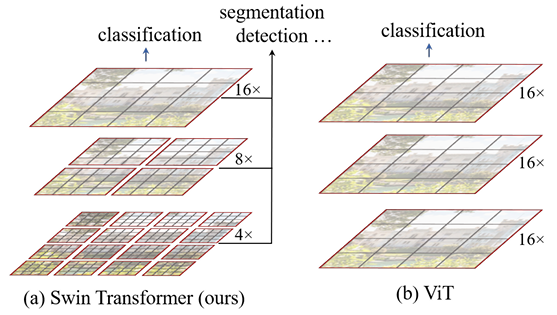
\includegraphics[width=1\linewidth]{Images/SWIN-vs-ViT.png}
    \caption{Swin Transformer vs Traditional Vision Transformer \cite{SwinPaper}}
    \label{fig:SwinVsViT}
\end{figure}

Figure \ref{fig:SwinVsViT} illustrates the differences between each transformer. The traditional ViT computes the global attention by breaking the image into fixed sized patches in every layer where every patch computes its relationship with every other patch in the image. This results in $N^2$ (N = number of patches) complexity. In comparison, the Swin transformer breaks the image into smaller windows, and computes local attention on each patch with dynamic patch sizes. The windows are merged and the dynamic patch size increases through each layer until there are no more windows to merge. Here the number of patches within each window are fixed so the overall complexity becomes $N\times M$ (N = number of windows, M = patches per window) which simplifies to $O(N)$. Swin performs similarly to how CNN models work with earlier layers learning low level image characteristics and the deeper layers learning the high level semantics.

\begin{figure}[!htb]
    \centering
    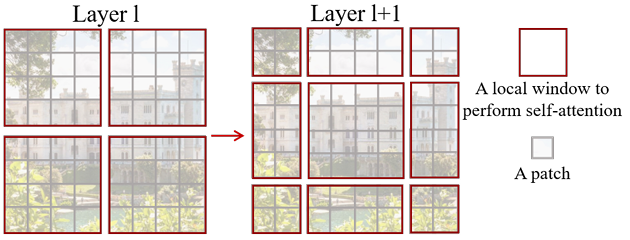
\includegraphics[width=1\linewidth]{Images/SwinShiftedWindow.png}
    \caption{Visualization of the shifted window mechanism in Swin transformer \cite{SwinPaper}}
    \label{fig:SwinShiftedWindow}
\end{figure}

While self-attention within each window learns the local context effectively, the model cannot learn the relationships between tokens that lie in separate windows. This is where the shifted window technique is employed. Shown in figure \ref{fig:SwinShiftedWindow}, the layer after the regular window partitioning uses the shifted window partition. This allows for overlap between the windows, enabling the model to learn a global context through the cross window connections. This means that in the model architecture, every other transformer block is a shifted window block as highlighted in figure \ref{fig:SwinArchitecture}.

\begin{figure} [!htb]
    \centering
    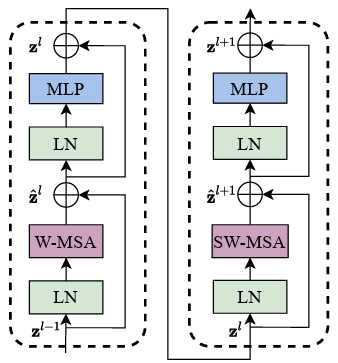
\includegraphics[width=0.5\linewidth]{Images/SwinArchitecture.png}
    \caption{Two successive Swin transformer blocks. W-MSA (Window MSA) followed by SW-MSA(Shifted Window MSA) \cite{SwinPaper}}
    \label{fig:SwinArchitecture}
\end{figure}

The paper for the Swin model highlights significantly improved performance over traditional ViTs and various other models for classification, detection, and segmentation. This was the deciding factor in testing the Swin model for our study.

\section{\textbf{Methodology}}
\subsection{\textbf{Data Analysis}}

\subsubsection{\textbf{Label Mapping (4 Classes)}}
SICAPv2 provides patch-level indicators for \{NC, G3, G4, G5, G4C\}. We use a fixed 4-class label space:
\{0,1,2,3\} = \{\text{NC}, \text{G3}, \text{G4}, \text{G5}\}, where G4C is merged into G4.

\textbf{Single-label verification:} we verified that every patch has exactly one active primary label among \{NC,G3,G4,G5\}. In particular, all rows in Train.xlsx satisfy this condition (9959/9959), and all rows in Test.xlsx satisfy this condition (2122/2122). Therefore, this is treated as \textbf{single-label} multi-class classification at the patch level.

\subsubsection{\textbf{Dataset Partitions and Split}}
We use the provided SICAPv2 partitions (Train.xlsx and Test.xlsx). The original training partition is split into train/validation using an \textbf{80/20 stratified split} with random\_state=42 (patch-level split).

\begin{table}[!htb]
\caption{Class Distributions After 4-Class Mapping}
\label{tab:vit_class_counts}
\centering
\begin{tabular}{lcccc}
\hline
\textbf{Split} & \textbf{NC} & \textbf{G3} & \textbf{G4} & \textbf{G5} \\
\hline
Train (full) & 3773 & 1829 & 3641 & 716 \\
Train (80\%) & 3018 & 1463 & 2913 & 573 \\
Val (20\%)   & 755  & 366  & 728  & 143 \\
Test         & 644  & 393  & 853  & 232 \\
\hline
\end{tabular}
\end{table}

\textit{Note:} the train/validation split is performed at the \textbf{patch level}. No patient/slide-level grouping is applied in this pipeline, so patches from the same patient may appear in both training and validation, which can make validation scores optimistic.

\subsection{\textbf{VGG-16 CNN Baseline Methodology}}

% -----------------------------
% OVERVIEW
% -----------------------------
\subsubsection{\textbf{Rationale}}
A VGG-16 convolutional neural network was implemented as a baseline to contextualize the performance of the Vision Transformer architectures. VGG-16 represents a well-established CNN architecture that has been widely used in medical image analysis, making it a suitable reference point for evaluating whether transformer-based approaches offer improvements for histopathology classification tasks.

% -----------------------------
% MODEL ARCHITECTURE
% -----------------------------
\subsubsection{\textbf{Model}}
The VGG-16 architecture (Configuration D) pretrained on ImageNet was used via \texttt{tf.keras.applications}. The original 1000-class ImageNet head was removed and replaced with a custom classifier:
\begin{itemize}
    \item \textbf{Pooling:} GlobalAveragePooling2D + GlobalMaxPooling2D (concatenated, 1024 features)
    \item \textbf{FC1:} Dense(1024, ReLU) + BatchNorm + Dropout(0.5)
    \item \textbf{FC2:} Dense(512, ReLU) + BatchNorm + Dropout(0.4)
    \item \textbf{FC3:} Dense(256, ReLU) + BatchNorm + Dropout(0.3)
    \item \textbf{Output:} Dense(4, softmax)
\end{itemize}
The concatenation of global average and max pooling captures both average activation patterns and salient features, providing a richer representation than either pooling method alone.

\textbf{Training from scratch (abandoned):} Initial experiments attempted to train VGG-16 from random initialization with BatchNormalization layers inserted after each convolutional layer. This approach resulted in training instability and poor convergence, with the model exhibiting strong bias toward the majority class (NC). Consequently, transfer learning from ImageNet weights was adopted.

% -----------------------------
% PREPROCESSING
% -----------------------------
\subsubsection{\textbf{Preprocessing}}
A TensorFlow \texttt{tf.data} pipeline was used for data loading and preprocessing:
\begin{enumerate}
    \item JPEG decode (3 channels)
    \item Resize to $224 \times 224$ pixels
    \item Cast to \texttt{float32}
    \item Normalize to $[0,1]$
    \item Batch (64) + prefetch
\end{enumerate}

\textbf{Data Augmentation.}
Extensive augmentation was applied during training to improve generalization and simulate stain variations common in histopathology:
\begin{enumerate}
    \item RandomHorizontalFlip
    \item RandomVerticalFlip
    \item Random 90$^\circ$ rotations (0$^\circ$, 90$^\circ$, 180$^\circ$, 270$^\circ$)
    \item ColorJitter (brightness=0.15, contrast=0.15, saturation=0.15, hue=0.05)
    \item RandomCrop (80--100\% of image) + resize to $224 \times 224$
    \item MixUp ($\alpha=0.2$)
\end{enumerate}
MixUp augmentation blends pairs of training images and their labels using a mixing coefficient, which has been shown to improve calibration and generalization in image classification tasks.

% -----------------------------
% TRAINING
% -----------------------------
\subsubsection{\textbf{Training}}
The model was trained with full fine-tuning of all convolutional layers. Class imbalance was addressed using inverse-frequency class weights with smoothing:
\[
w_c = (1 - \epsilon) \cdot \frac{N}{C \cdot n_c} + \epsilon
\]
where $N$ is the total samples, $C$ is the number of classes, $n_c$ is the count for class $c$, and $\epsilon = 0.1$ is a smoothing factor. The resulting weights were $\{w_0, w_1, w_2, w_3\} = \{0.694, 1.325, 0.715, 3.230\}$ for $\{\text{NC}, \text{G3}, \text{G4}, \text{G5}\}$.

\textbf{Learning Rate Schedule.}
A warmup followed by cosine decay schedule was employed:
\[
\text{lr}(t) =
\begin{cases}
\text{lr}_{\text{init}} \cdot \frac{t}{T_{\text{warmup}}} & \text{if } t < T_{\text{warmup}} \\[6pt]
\text{lr}_{\text{min}} + \frac{1}{2}(\text{lr}_{\text{init}} - \text{lr}_{\text{min}})\left(1 + \cos\left(\pi \cdot \frac{t - T_{\text{warmup}}}{T_{\text{total}} - T_{\text{warmup}}}\right)\right) & \text{otherwise}
\end{cases}
\]
with $\text{lr}_{\text{init}} = 1 \times 10^{-4}$, $\text{lr}_{\text{min}} = 1 \times 10^{-7}$, and $T_{\text{warmup}} = 5$ epochs.

\textbf{Optimization settings:}
\begin{itemize}
    \item \textbf{Optimizer:} AdamW (weight decay $= 1 \times 10^{-4}$)
    \item \textbf{Loss:} Categorical Cross-Entropy with label smoothing ($\epsilon = 0.1$)
    \item \textbf{Callbacks:} EarlyStopping (patience=15, restore best weights), ModelCheckpoint
    \item \textbf{Max Epochs:} 100
\end{itemize}

% -----------------------------
% EVALUATION
% -----------------------------
\subsubsection{\textbf{Evaluation}}
Model evaluation was performed on the held-out test set (Test.xlsx). To improve prediction robustness, \textbf{Test-Time Augmentation (TTA)} was applied by averaging softmax predictions over 5 augmented versions of each test image (original + 4 augmented copies with random flips and rotations). Final class predictions were obtained by taking the argmax of the averaged probabilities.


\subsection{\textbf{Vision Transformer (ViT) Methodology}}

% -----------------------------
% ViT FROM SCRATCH
% -----------------------------
\subsubsection{\textbf{ViT Trained From Scratch}}

\textbf{Model.}
A Vision Transformer was implemented in Keras and trained from random initialization for 4-class patch-level classification (NC, G3, G4, G5). The model configuration is:
\begin{itemize}
    \item \textbf{Input Image Resolution:} $224\times224$ pixels
    \item \textbf{Patch Size:} $16\times16$ pixels
    \item \textbf{Number of Tokens:} $14\times14 = 196$
    \item \textbf{Projection Dimension:} 64
    \item \textbf{Transformer Blocks:} 8
    \item \textbf{Attention Heads:} 4
    \item \textbf{Classifier:} GlobalAveragePooling over tokens + MLP head + 4-way softmax
\end{itemize}

\textbf{Preprocessing.}
A TensorFlow pipeline was used to handle data loading and preprocessing:
\begin{enumerate}
    \item JPEG decode
    \item Resize((224,224))
    \item Cast to \texttt{float32}
    \item Normalize to $[0,1]$
    \item Batch (32) + prefetch
\end{enumerate}
Training data is shuffled; validation and test are not shuffled. Data augmentation is applied inside the model during training using:
\begin{enumerate}
    \item RandomHorizontalFlip
    \item RandomRotation(0.05)
    \item RandomZoom(0.1)
    \item RandomContrast(0.1)
    \item RandomTranslation(0.05, 0.05)
\end{enumerate}

\textbf{Training.}
The model was trained with class imbalance handling enabled using balanced class weights
($\{w_0,w_1,w_2,w_3\}=\{0.6599, 1.3614, 0.6837, 3.4760\}$ for \{NC,G3,G4,G5\}).
Optimization and training settings were:
\begin{itemize}
    \item \textbf{Optimizer:} AdamW (lr=$1\times10^{-4}$, weight decay=$1\times10^{-5}$)
    \item \textbf{Loss:} Sparse Categorical Cross-Entropy
    \item \textbf{Callbacks:} EarlyStopping (patience=5) and ReduceLROnPlateau (factor=0.5, patience=3, min lr=$1\times10^{-6}$)
    \item \textbf{Max Epochs:} 40 (EarlyStopping typically stops earlier)
\end{itemize}

% -----------------------------
% PRETRAINED VIT-B/16
% -----------------------------
\subsubsection{\textbf{Pretrained ViT-B/16 (Transfer Learning)}}

\textbf{Model.}
A ViT-B/16 backbone pretrained on ImageNet was used via \texttt{vit-keras}. The original classifier head was removed and replaced with a custom 4-class head:
\begin{itemize}
    \item Dense(256, ReLU)
    \item Dropout(0.5)
    \item Dense(4, softmax)
\end{itemize}

\textbf{Preprocessing.}
The same TensorFlow pipeline is used to produce images normalized to $[0,1]$. For compatibility with pretrained ViT representations, inputs are scaled to $[-1,1]$ before the backbone using:
\[
x' = 2x - 1
\]

\textbf{Training.}
Training follows a two-stage procedure with class weights enabled (same weights as the scratch ViT):
\begin{enumerate}
    \item \textbf{Stage 1 (Frozen backbone):} Freeze the entire backbone and train only the new head using Adam (lr=$10^{-3}$), up to 10 epochs.
    \item \textbf{Stage 2 (Fine-tuning):} Unfreeze the backbone and fine-tune only the last portion of layers by keeping all but the last 40 layers frozen. Fine-tuning uses AdamW (lr=$10^{-5}$, weight decay=$10^{-6}$), up to 10 epochs.
\end{enumerate}
In both stages, EarlyStopping (patience=5) and ReduceLROnPlateau are applied.


\subsection{\textbf{Swin Transformer Methodology}}
\subsubsection{\textbf{Model}}
A Swin backbone pretrained on ImageNet-22k and then fine-tuned on ImageNet-1k was used. We replaced the classification head of the backbone with a new 4-class head and fine-tuned it on the SICAPv2 dataset with the classes Non-cancerous, G3, G4, and G5. The Swin backbone had the following configuration:
\begin{itemize}
    \item \textbf{Model Size:} Base $\sim$ 88 million parameters
    \item \textbf{Patch Size:} $4\times 4$ pixels
    \item \textbf{Window Size:} $7\times 7$ patches
    \item \textbf{Input Image Resolution:} $224\times 224$ pixels
\end{itemize}

\subsubsection{\textbf{Preprocessing}}
A PyTorch transform pipeline with a data loader was used to handle all data preprocessing. The processing pipeline for training is as follows:
\begin{enumerate}
    \item Resize((224,224))
    \item RandomHorizontalFlip(p=0.5)
    \item RandomVerticalFlip(p=0.5)
    \item RandomRotation(degrees=180)
    \item ColorJitter
    \item To Tensor
    \item Normalize
\end{enumerate}
Every time the data loader sent an image to the model during training, it was resized, converted to a tensor, and normalized. The image was randomly flipped vertically or horizontally with a 50\% probability, rotated anywhere from -180$^\circ$ to 180$^\circ$, and had its colors slightly tweaked as a means of data augmentation. For testing and validation, only resize, tensor conversion, and normalization steps were applied.

\subsubsection{\textbf{Training}}
The model was fine-tuned with a weighted sparse categorical cross-entropy loss function to account for class imbalances. The following hyperparameters were used during model training:
\begin{itemize}
    \item \textbf{Optimizer: }Adam
    \item \textbf{Learning Rate: } $1\times10^{-5}$
    \item \textbf{Weight Decay: } $1\times10^{-6}$
    \item \textbf{Loss: } Weighted Sparse Categorical Cross-Entropy
    \item \textbf{Epochs: } 10
\end{itemize}
Here the weight decay adds an L2 regularization term to penalize the model from overfitting to the training data. A two-stage training process was used to fine-tune the model. First, the entire backbone was frozen with only the classification head learning the new data. Once the first stage converged, the last two layers in the backbone were unfrozen and the model was retrained. In each stage, the hyperparameters remained the same. This is a common practice when doing transfer learning to improve performance.


\section{\textbf{Experiments and Results}}
\subsection{\textbf{VGG-16 CNN Baseline Experiments and Results}}

This section presents the evaluation metrics, confusion matrix, and ROC curves for the VGG-16 CNN baseline on the SICAPv2 test set.

\begin{table}[!htb]
\caption{VGG-16 CNN Baseline Test Performance Metrics}
\label{tab:VGG16Results}
\centering
\begin{tabular}{lc}
\hline
\textbf{Metric} & \textbf{VGG-16} \\
\hline
Accuracy & 0.7771 \\
Macro Precision & 0.7478 \\
Macro Recall & 0.7369 \\
Macro F1 & 0.7414 \\
Macro AUC (OvR) & 0.9373 \\
QWK & 0.7910 \\
\hline
\end{tabular}
\end{table}

Table \ref{tab:VGG16Results} summarizes the test performance of the VGG-16 baseline.

\begin{figure}[!htb]
    \centering
    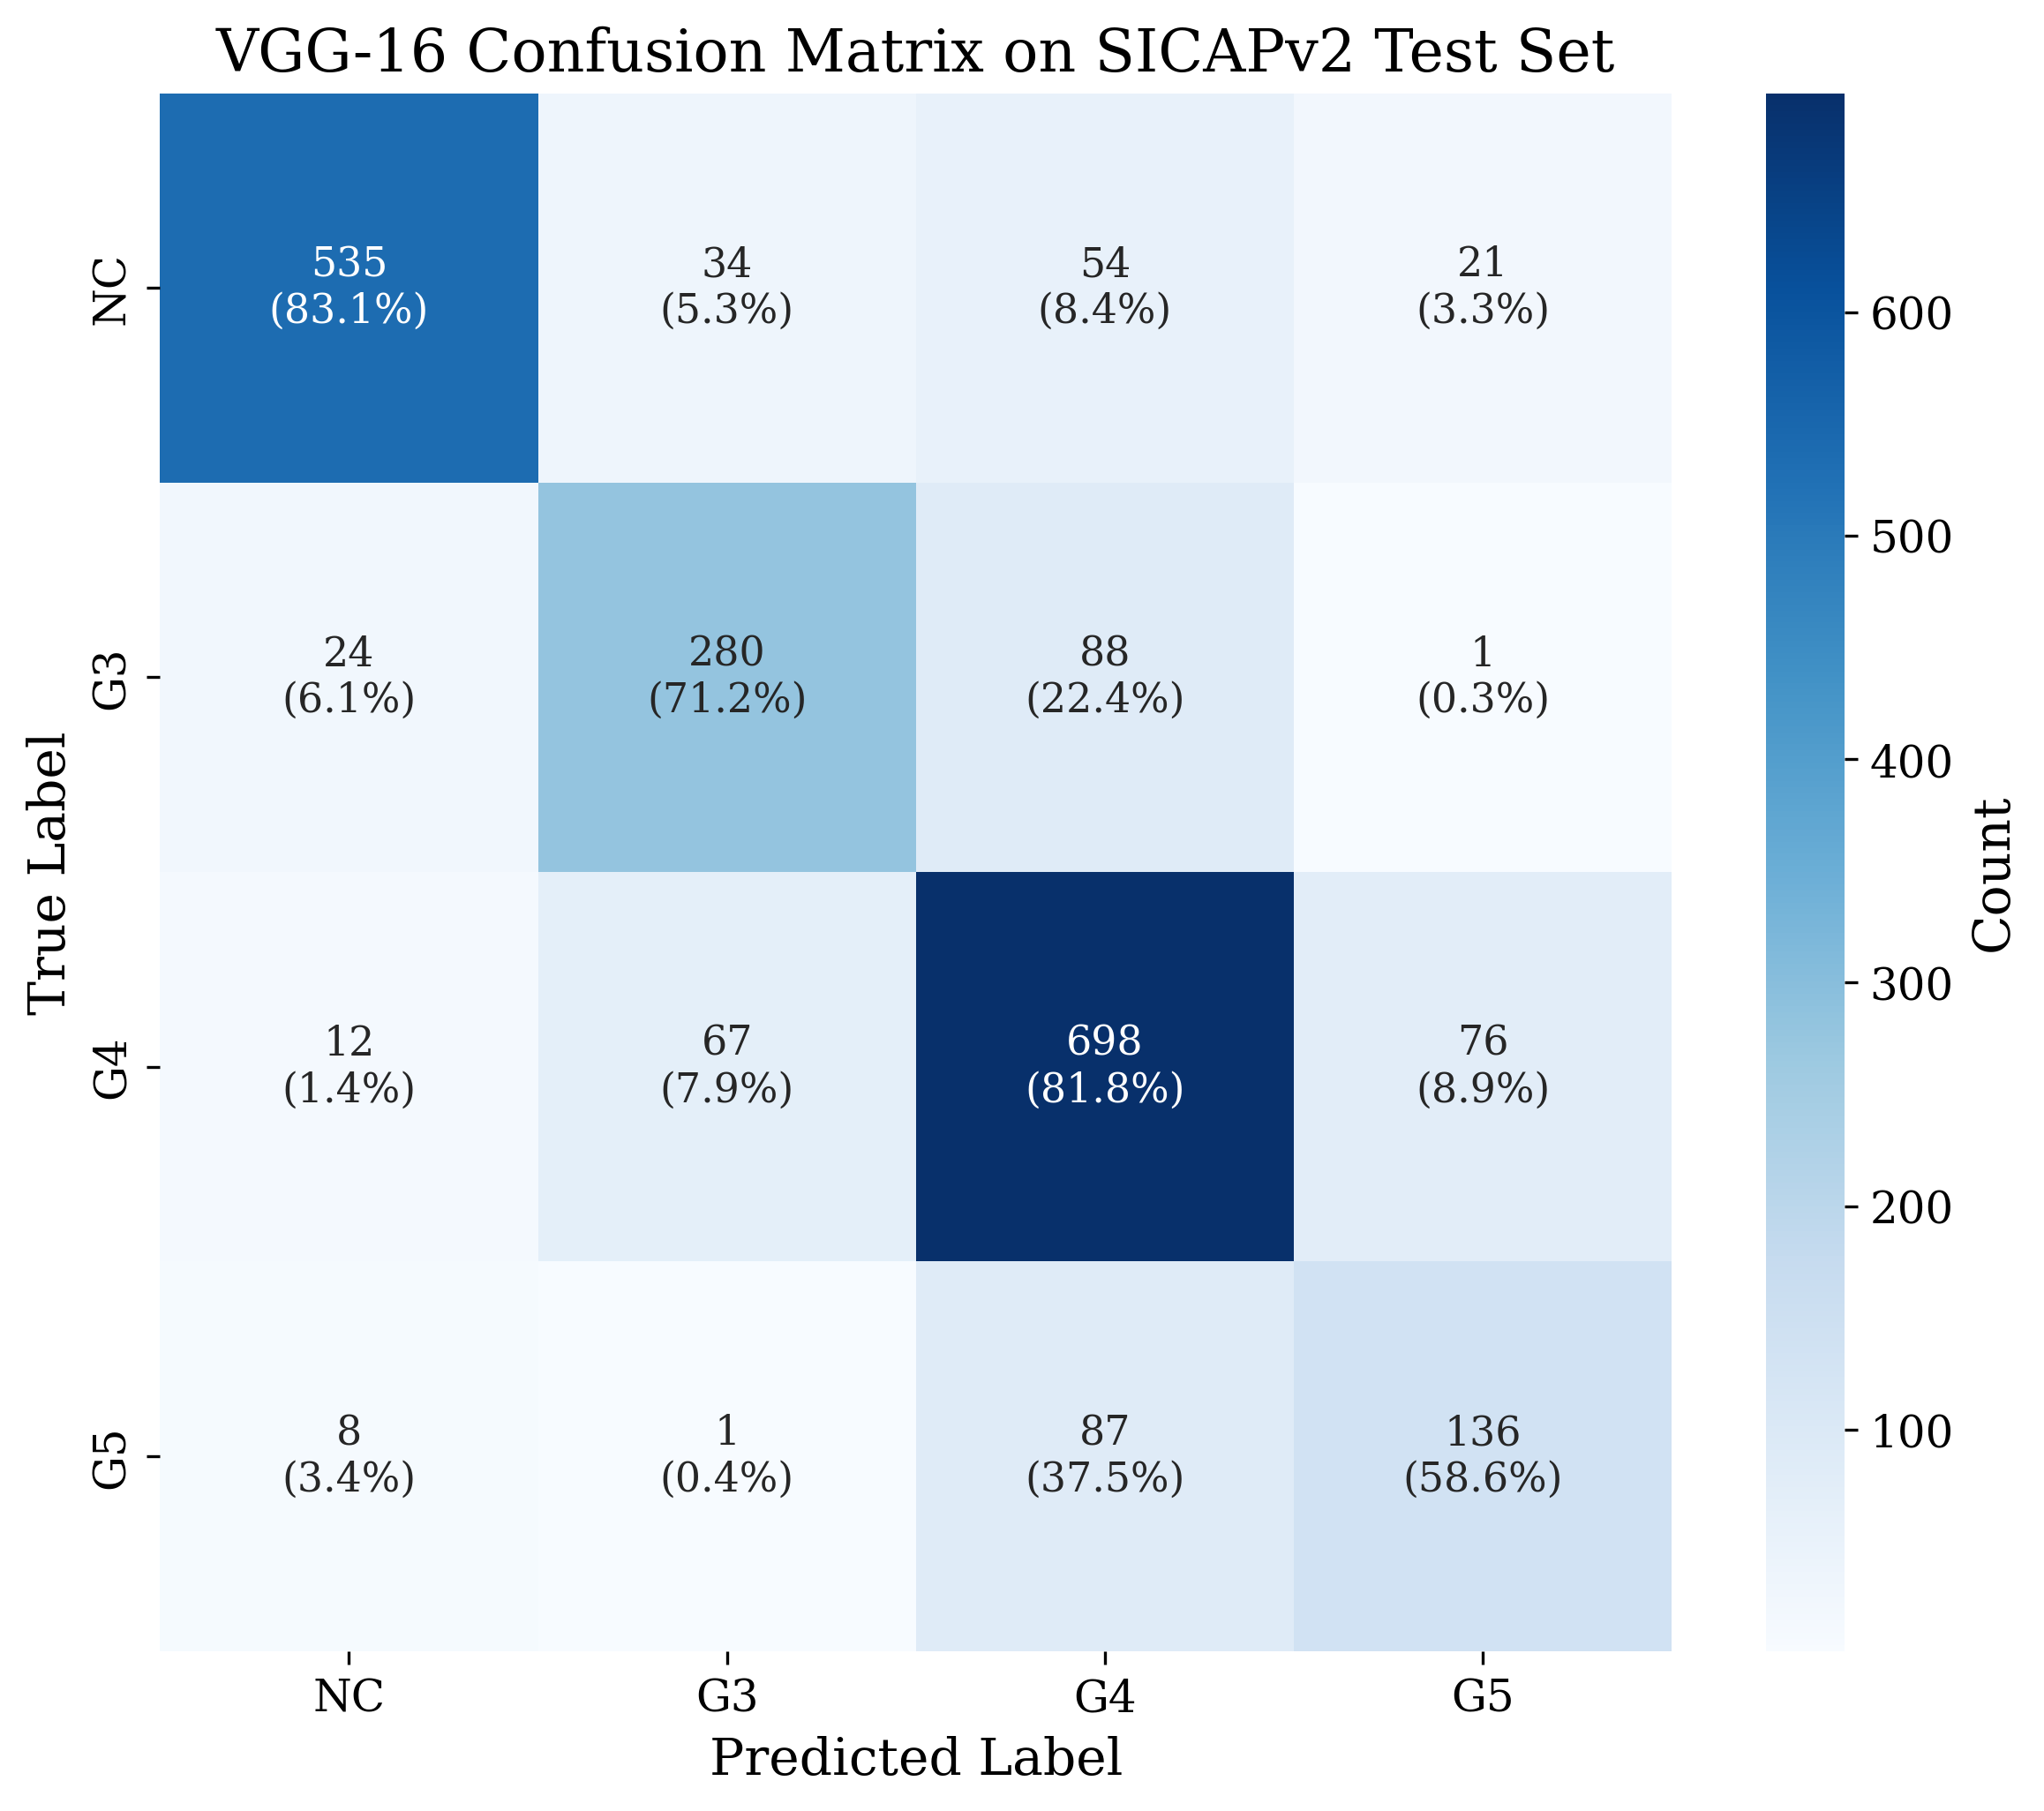
\includegraphics[width=1\linewidth]{Images/vgg16_confusion_matrix.png}
    \caption{VGG-16 Gleason Classification Confusion Matrix}
    \label{fig:VGG16ConfusionMatrix}
\end{figure}

Figure \ref{fig:VGG16ConfusionMatrix} shows the confusion matrix for the VGG-16 baseline. The diagonal entries show the number of correct classifications made by the model. Off-diagonal entries show misclassifications.

\begin{figure}[!htb]
    \centering
    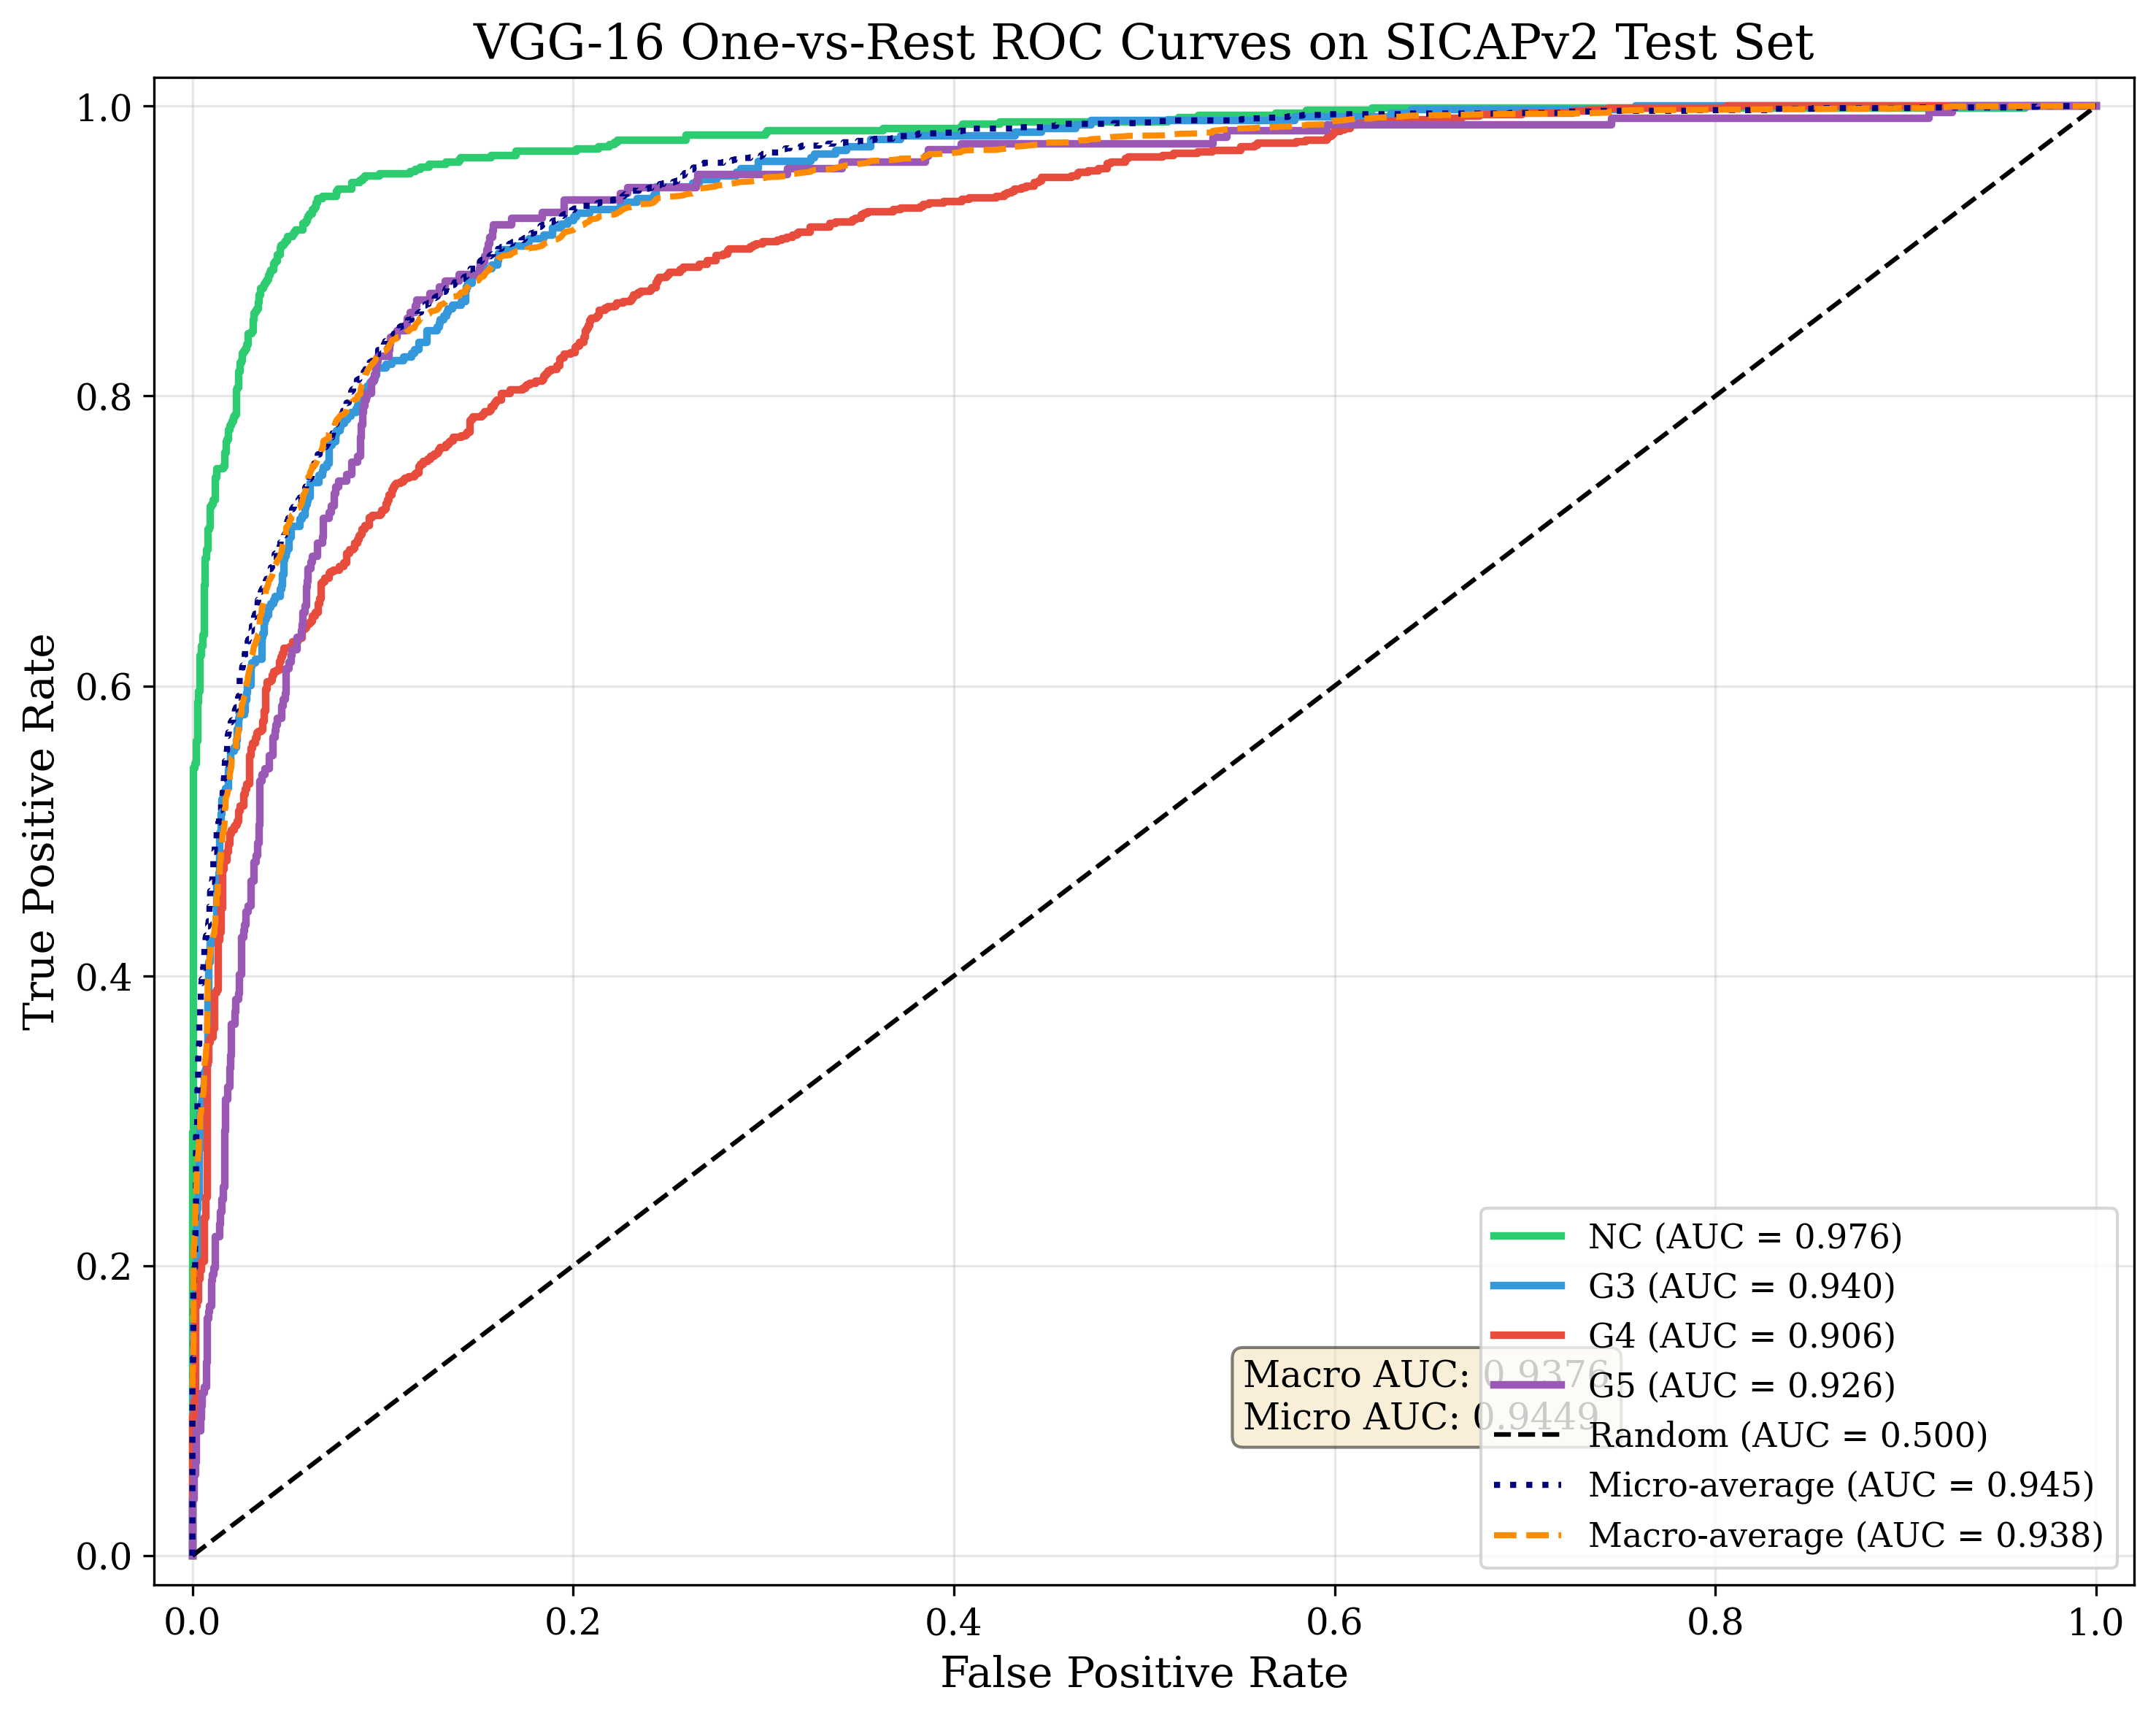
\includegraphics[width=1\linewidth]{Images/vgg16_roc_curves.png}
    \caption{VGG-16 One-vs-Rest ROC Curves (Macro AUC = 0.937)}
    \label{fig:VGG16ROC}
\end{figure}

Figure \ref{fig:VGG16ROC} displays the one-vs-rest ROC curves for each class. Each curve illustrates the model's true positive rate against the false positive rate for a given Gleason grade. The model reports AUC of 0.976 for non-cancerous cases, 0.940 for Gleason grade 3, 0.906 for Gleason grade 4, and 0.926 for Gleason grade 5.

\subsection{\textbf{ViT Experiments and Results}}

The scratch ViT and ViT-B/16 metrics are computed on the test set with fixed class order [NC, G3, G4, G5]. We report accuracy, macro precision/recall/F1, macro OvR ROC-AUC, quadratic weighted kappa (QWK), and confusion matrices.

\begin{table}[!htb]
\caption{Test Performance Comparison (ViT Models)}
\label{tab:vit_results}
\centering
\begin{tabular}{lcc}
\hline
\textbf{Metric} & \textbf{Scratch ViT} & \textbf{Pretrained ViT-B/16} \\
\hline
Accuracy & 0.4760 & 0.7215 \\
Macro Precision & 0.5547 & 0.6821 \\
Macro Recall & 0.5080 & 0.6739 \\
Macro F1 & 0.4726 & 0.6707 \\
Macro AUC (OvR) & 0.8150 & 0.9074 \\
QWK & 0.6037 & 0.7965 \\
\hline
\end{tabular}
\end{table}

Table \ref{tab:vit_results} summarizes test performance for the ViT trained from scratch and the pretrained ViT-B/16.
The pretrained model performs better across all metrics, improving accuracy (0.4760$\rightarrow$0.7215) and macro F1 (0.4726$\rightarrow$0.6707), which indicates stronger overall correctness and more balanced performance across classes.
Macro precision/recall/F1 are particularly important here because SICAPv2 is class-imbalanced; these metrics reduce the chance that high performance is driven mainly by the majority class.
The higher macro OvR AUC for the pretrained model (0.8150$\rightarrow$0.9074) also suggests better separability between Gleason grades, while the higher QWK (0.6037$\rightarrow$0.7965) indicates that remaining mistakes tend to be closer in grade rather than extreme mismatches.

\begin{figure}[!htb]
    \centering
    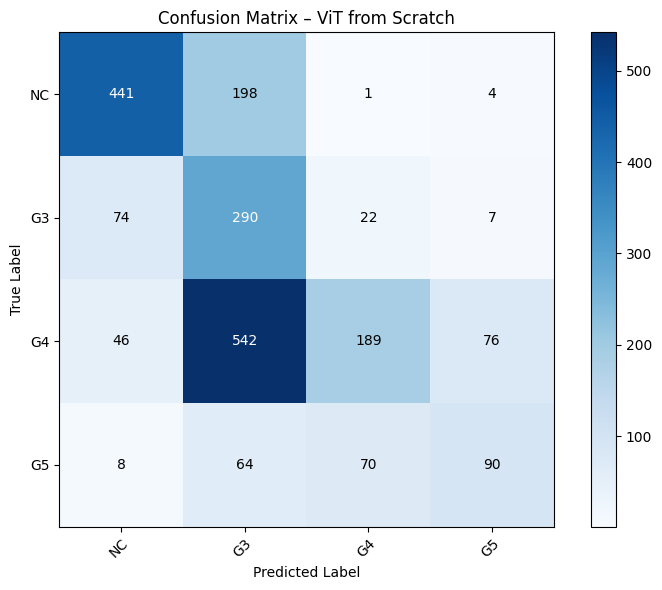
\includegraphics[width=1\linewidth]{Images/scrtch_vit_heatmjap.png}
    \caption{ViT from Scratch Classification Confusion Matrix}
    \label{fig:scrtch_vit_heatmjap}
\end{figure}

Figure \ref{fig:scrtch_vit_heatmjap} shows that the scratch ViT most frequently confuses G4 with G3 (large off-diagonal mass), which reduces macro F1 despite reasonable performance on NC.


\begin{figure}[!htb]
    \centering
    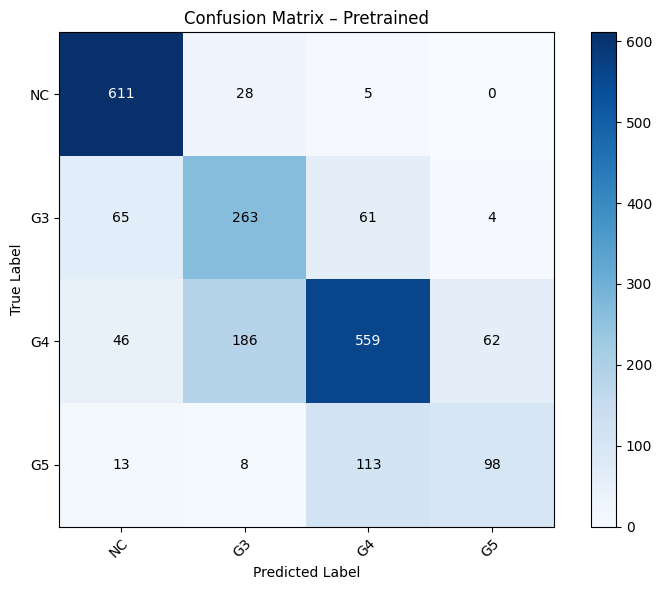
\includegraphics[width=1\linewidth]{Images/cm_pre.png}
    \caption{ViT-B/16 Classification Confusion Matrix}
    \label{fig:cm_pre}
\end{figure}

Figure \ref{fig:cm_pre} shows improved overall classification compared to the scratch ViT, with a stronger diagonal across all classes and reduced confusion between neighboring Gleason grades.

\begin{figure}[!htb]
    \centering
    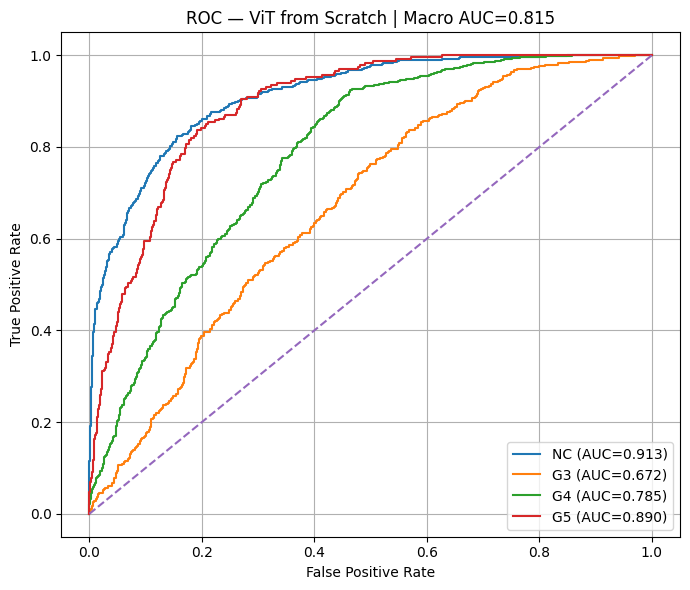
\includegraphics[width=1\linewidth]{Images/auc_scracth.png}
    \caption{One-vs-Rest ROC curves for the ViT trained from scratch (Macro AUC = 0.815).}
    \label{fig:auc_scracth}
\end{figure}
Figure \ref{fig:auc_scracth} shows the one-vs-rest ROC curves for each class (NC, G3, G4, G5) for the scratch ViT. Curves closer to the top-left indicate better discrimination, while the dashed diagonal represents chance-level performance.

\begin{figure}[!htb]
    \centering
    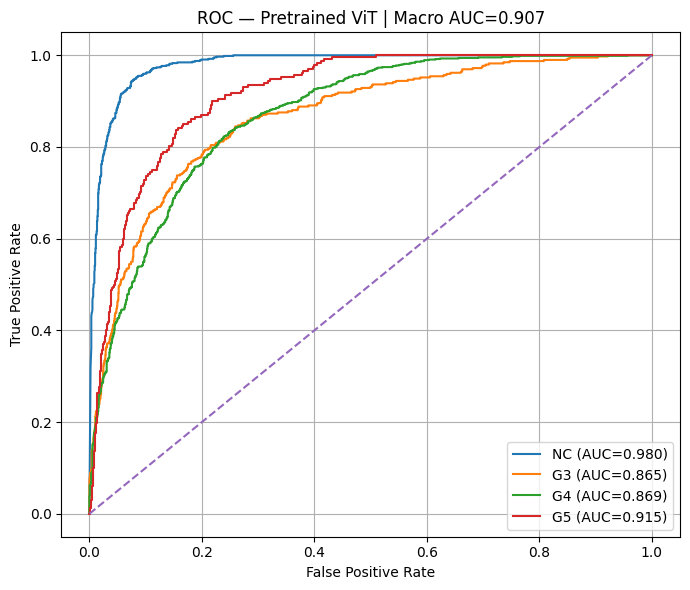
\includegraphics[width=1\linewidth]{Images/pre_auc.png}
    \caption{One-vs-Rest ROC curves for the pretrained ViT-B/16 (Macro AUC = 0.907).}
    \label{fig:pre_auc}
\end{figure}
Figure \ref{fig:pre_auc} shows the ROC curves for the pretrained ViT-B/16. Compared to the scratch model, the curves are generally higher, consistent with the higher macro AUC reported in Table \ref{tab:vit_results}.


\begin{figure}[!htb]
    \centering
    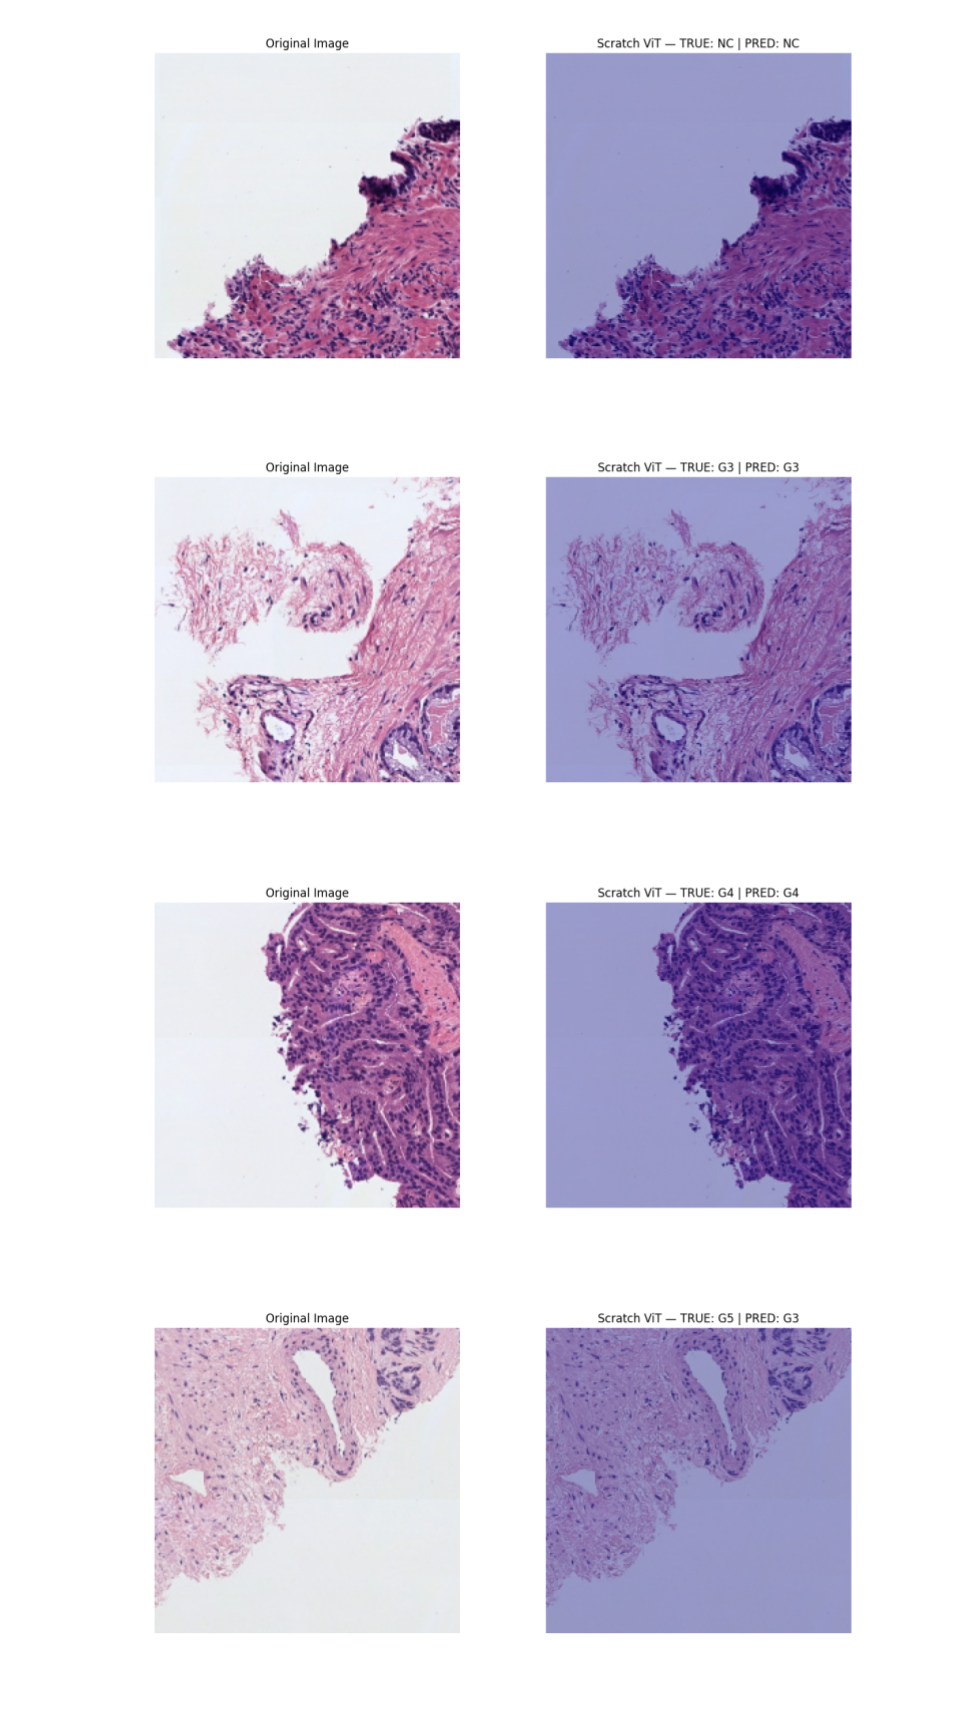
\includegraphics[width=1\linewidth]{Images/scratch_grad.png}
    \caption{Grad-CAM-style visualizations for the ViT trained from scratch. Each row shows one representative test patch per class (NC, G3, G4, G5), with the original image (left) and the heatmap overlay (right).}
    \label{fig:ViTScratchGradCAM}
\end{figure}

\begin{figure}[!htb]
    \centering
    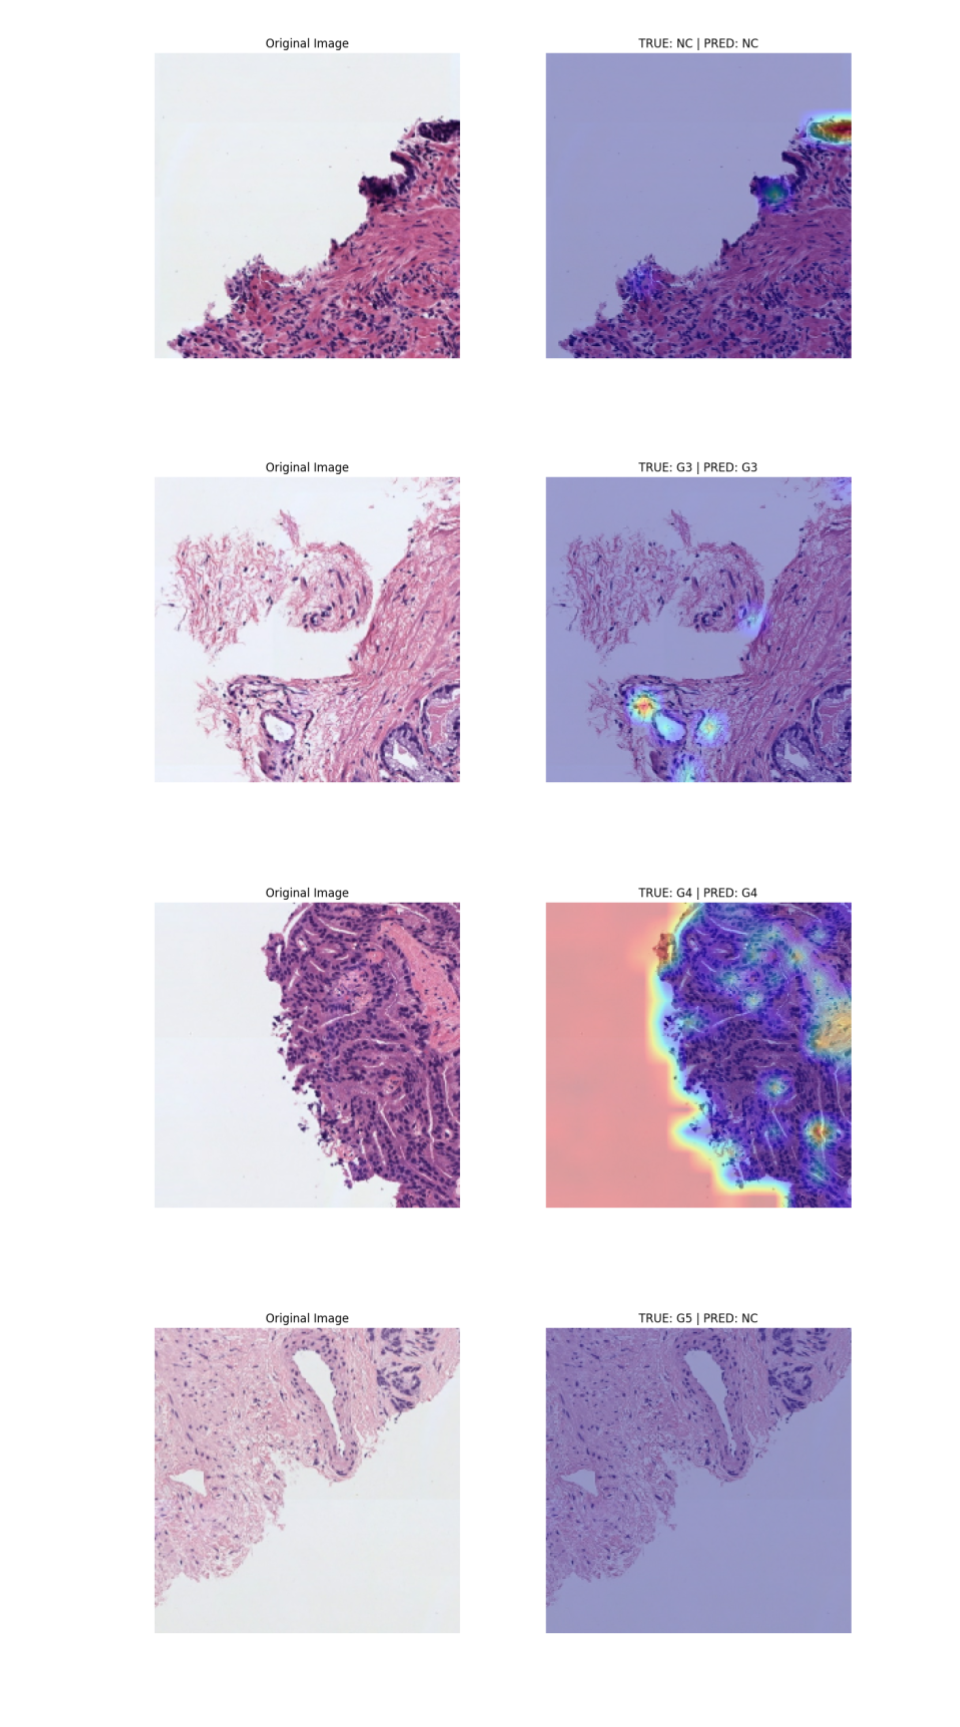
\includegraphics[width=1\linewidth]{Images/pretrained_grad.png}
    \caption{Grad-CAM-style visualizations for the pretrained ViT-B/16. Each row shows one representative test patch per class (NC, G3, G4, G5), with the original image (left) and the heatmap overlay (right).}
    \label{fig:ViTPreGradCAM}
\end{figure}
Figures \ref{fig:ViTScratchGradCAM} and \ref{fig:ViTPreGradCAM} show the corresponding visualizations for our ViT models. For the scratch ViT, we compute a gradient-based patch attribution map using gradients with respect to the token sequence representation (a $14\times14$ patch grid) and then upsample it to $224\times224$. For the pretrained ViT-B/16, we generate Grad-CAM-like heatmaps using gradients with respect to the patch-embedding convolution activations (spatial $14\times14$), and overlay the resulting heatmap on the original patch.

\subsection{\textbf{Swin Experiments and Results}}
This section presents the evaluation metrics, confusion matrix, ROC curves, and Grad-CAM visualizations for the Swin Transformer model on the SICAPv2 test set.

\begin{table}[!htb]
\caption{Swin Test Performance Metrics}
\label{tab:SwinResults}
\centering
\begin{tabular}{lc}
\hline
\textbf{Metric} & \textbf{Swin} \\
\hline
Accuracy & 0.8016\\
Macro Precision & 0.7753  \\
Macro Recall & 0.7793 \\
Macro F1 & 0.7751\\
Macro AUC (OvR) & 0.9487  \\
QWK & 0.8506 \\
\hline
\end{tabular}
\end{table}

Table \ref{tab:SwinResults} shows the overall accuracy, quadratic weighted kappa, and macro precision, recall, F1, and AUC. Overall, the model shows consistent performance over all the metrics.

\begin{figure}[!htb]
    \centering
    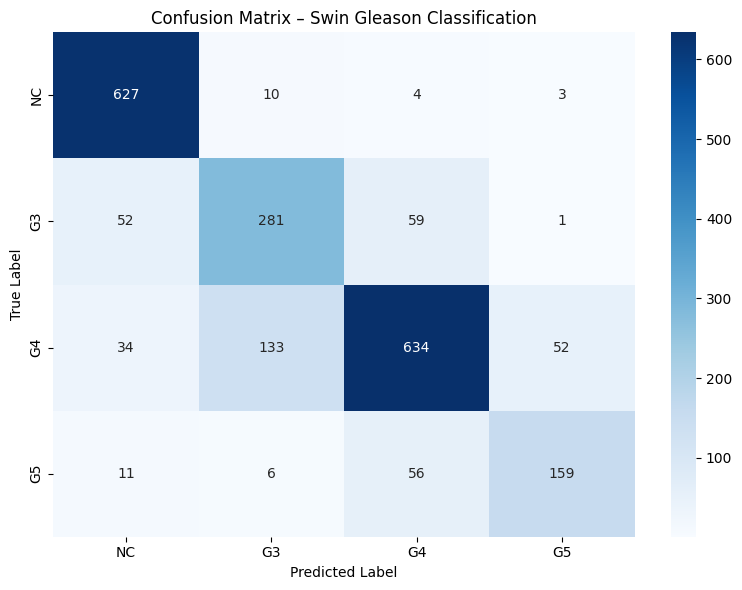
\includegraphics[width=1\linewidth]{Images/SwinConfusionMatrix.png}
    \caption{Swin Gleason Classification Confusion Matrix}
    \label{fig:SwinConfusionMatrix}
\end{figure}

Figure \ref{fig:SwinConfusionMatrix} shows the confusion matrix for the Swin Transformer. The diagonal entries show the number of correct classifications made by the model. Off-diagonal entries show misclassifications.

\begin{figure}[!htb]
    \centering
    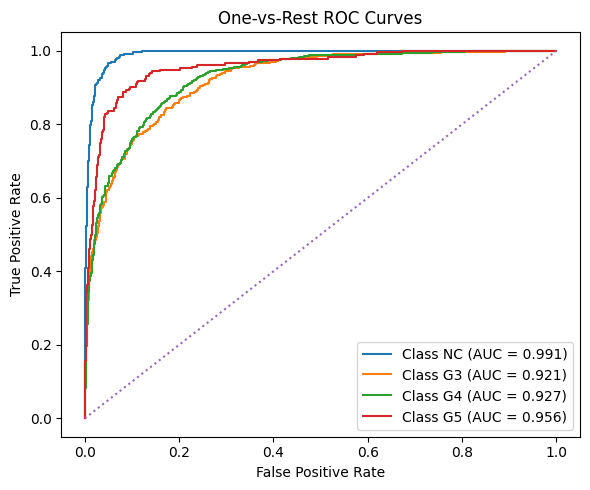
\includegraphics[width=1\linewidth]{Images/SwinROC.png}
    \caption{Swin Gleason Classification OvR ROC Curves}
    \label{fig:SwinROC}
\end{figure}

Figure \ref{fig:SwinROC} displays the one-vs-rest ROC curves for each class. Each curve illustrates the model's true positive rate against the false positive rate for a given Gleason grade. A perfect model performance is defined by an AUC of 1.000. The model reports AUC of 0.991 for non-cancerous cases, 0.921 for Gleason grade 3, 0.927 for Gleason grade 4, and 0.956 for Gleason grade 5.

\begin{figure}[!htb]
    \centering
    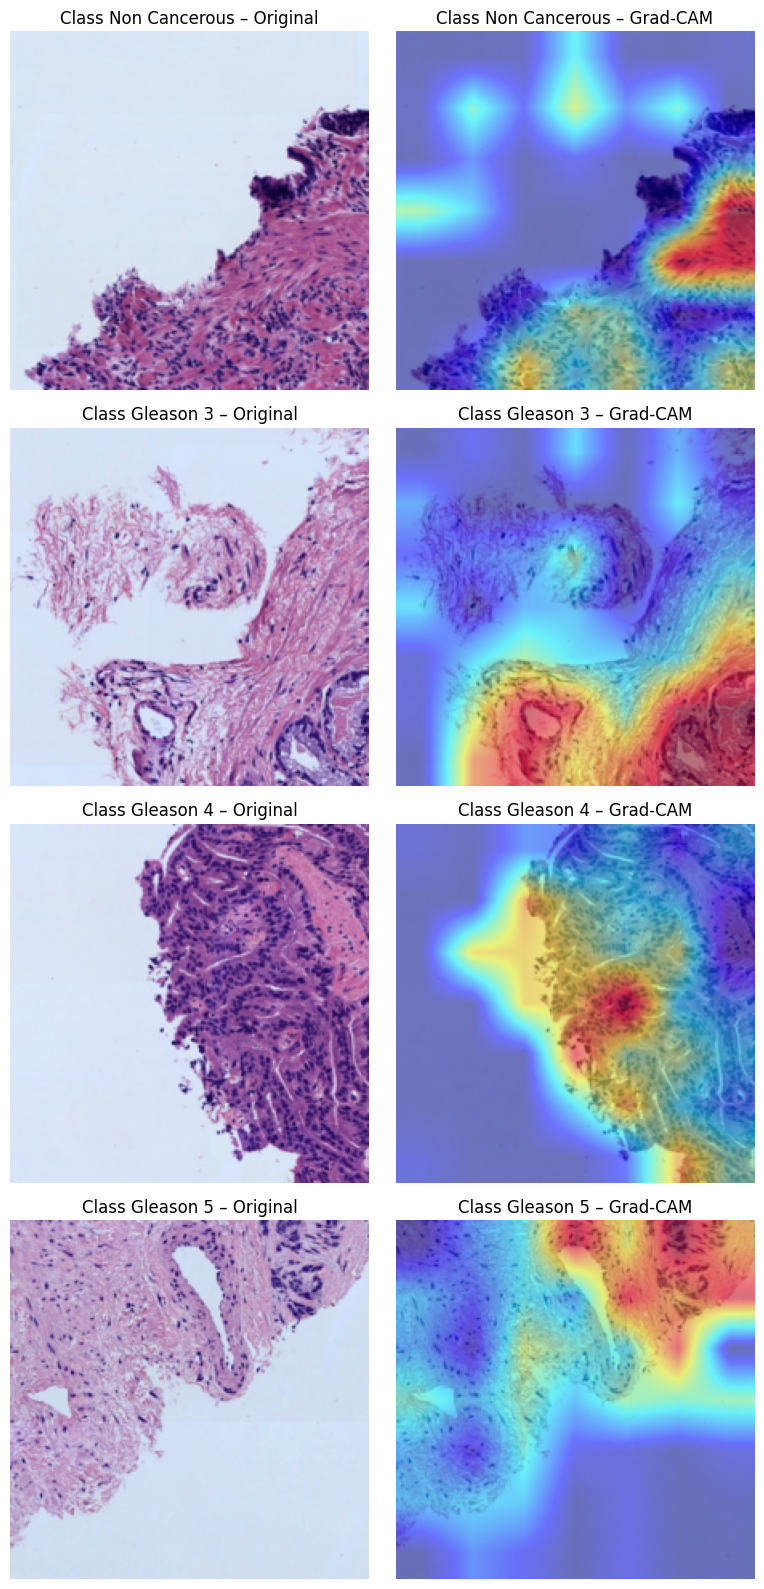
\includegraphics[width=1\linewidth]{Images/SwinGradCam.png}
    \caption{Swin Transformer Gleason score Grad-CAM outputs and comparisons with the original images}
    \label{fig:SwinGradCAM}
\end{figure}

Figure \ref{fig:SwinGradCAM} shows the Grad-CAM results for the model. The left column shows the original image with the right column showing the Grad-CAM heatmap overlay. The heatmaps show the regions of interest that the model uses to make classifications.



\section{\textbf{Discussion}}

\subsection{\textbf{VGG-16 CNN Baseline Performance Analysis}}
The VGG-16 CNN baseline shows strong overall performance across the evaluation metrics. The accuracy score of 77.71\% demonstrates that the fine-tuned convolutional architecture effectively learns discriminative features for Gleason grading. A quadratic weighted kappa score of 0.7910 indicates substantial agreement, suggesting that the majority of misclassifications occur between neighboring grades rather than extreme mismatches.

The macro precision, recall, and F1 scores (0.7478, 0.7369, 0.7414) show that the model performs relatively evenly across all classes without strong bias toward the majority classes. This is notable given the class imbalance in SICAPv2, where G5 comprises only 7.2\% of the training set. The high macro AUC score of 0.9373 confirms that the model achieves strong separability between all Gleason grades.

The per-class AUC values reveal that NC achieves the highest discriminability (0.976), reflecting the distinct morphological differences between cancerous and non-cancerous tissue. G4 has the lowest per-class AUC (0.906), which is expected given its intermediate position between G3 and G5 in the Gleason grading spectrum.

The confusion matrix shows that most predictions lie along the diagonal, with per-class recall of 83.1\% (NC), 71.2\% (G3), 81.8\% (G4), and 58.6\% (G5). The primary source of confusion is between G5 and G4, where 37.5\% of G5 samples are misclassified as G4. This pattern is consistent with the morphological similarity between high-grade patterns and the limited G5 training samples. Misclassifications between non-adjacent grades (e.g., NC to G5) are rare, indicating that the model captures the ordinal structure of Gleason grades.

Overall, the VGG-16 baseline demonstrates that traditional CNN architectures remain competitive for patch-level Gleason grading when properly fine-tuned with transfer learning. The model outperforms both the scratch ViT and pretrained ViT-B/16 in terms of accuracy and macro F1, while achieving comparable QWK. However, the Swin Transformer surpasses VGG-16 across all metrics, suggesting that the hierarchical attention mechanism provides additional benefits for histopathology classification. The VGG-16 results establish a strong CNN reference point for evaluating the transformer-based approaches in this project.

\subsection{\textbf{ViT from Scratch Performance Analysis}}
The ViT trained from scratch shows moderate overall performance across the evaluation metrics. The accuracy score of 47.60\% indicates that the model learns meaningful patterns, but still makes frequent classification errors. The macro precision, recall, and F1 scores (0.5547, 0.5080, 0.4726) suggest that performance is uneven across classes, which is common in imbalanced and fine-grained Gleason grading tasks. The quadratic weighted kappa (QWK) score of 0.6037 suggests that many of the model's mistakes occur between neighboring grades rather than extreme mismatches.

The macro AUC score of 0.8150 further shows reasonable class separability, but the per-class ROC curves indicate that intermediate grades (G3 and G4) remain more difficult to distinguish compared to NC and G5. The confusion matrix supports this behavior, where a substantial portion of errors occur between adjacent grades, particularly confusion between G4 and G3.

Finally, the Grad-CAM visualizations provide interpretability by highlighting which regions influence predictions. While the model often focuses on tissue structures relevant to grading, the weaker overall performance suggests that attention is not consistently concentrated on the most discriminative cancer patterns, especially for intermediate grades.

Overall, the scratch ViT provides a useful baseline for transformer-based Gleason grading on SICAPv2, but its performance and confusion patterns indicate that training from random initialization is less effective for separating neighboring Gleason grades.


\subsection{\textbf{ViT-B/16 Performance Analysis}}
The pretrained ViT-B/16 model shows substantially stronger overall performance across all evaluation metrics. The accuracy score of 72.15\% demonstrates that transfer learning improves classification reliability on SICAPv2 patches. The macro precision, recall, F1 scores, and QWK score (0.6821, 0.6739, 0.6707, 0.7965) also indicate more balanced performance across the four classes compared to the scratch model.


The macro AUC score of 0.9074 confirms improved separability, and the ROC curves show consistently higher per-class AUC values compared to the scratch ViT. The confusion matrix shows that most predictions lie along the diagonal, with remaining errors mostly between adjacent grades (e.g., G3 vs G4 and G4 vs G5), which is expected given patch-level ambiguity and overlap between neighboring Gleason patterns.


The Grad-CAM visualizations also help interpret model behavior by highlighting regions that contribute to predictions. With high-level inspection, the pretrained model generally places attention on relevant tissue morphology and cancer-associated patterns, supporting the idea that it learns clinically meaningful cues rather than relying on irrelevant features.

Overall, the pretrained ViT-B/16 is more reliable than the scratch ViT for patch-level Gleason grading on SICAPv2. While some confusion between neighboring grades remains, transfer learning improves both separability and consistency across classes, making pretrained ViT a stronger candidate for automated grading support.

\subsection{\textbf{Swin Performance Analysis}}
The Swin model shows relatively high overall performance across the evaluation metrics. The accuracy score of 80.16\% shows that the model consistently predicts the inputs as the correct class. A quadratic weighted kappa score of 0.8506, which is higher than the accuracy, indicates that many of the misclassifications made by the model belong to classes close to the target class.

The macro precision, recall, and F1 scores (0.7753, 0.7793, 0.7751) show that the model performs relatively evenly across all the classes without showing any bias towards a single class. This claim is further backed by the high macro AUC score of 0.9487, showing that the model can correctly differentiate between every class. The per-class AUC of the Gleason 3 and Gleason 4 classes was lower than that of the non-cancerous and Gleason 5 classes, indicating that the model struggles more to differentiate Gleason 3 and Gleason 4 from the other classes.

The confusion matrix further shows the model's capability to correctly predict each class, as a majority of the predictions lie on the diagonal. Supporting the results indicated by the quadratic weighted kappa, most misclassifications are made between adjacent classes such as G3 vs G4 or G4 vs G5. This result is expected, as histopathology images contain many ambiguous regions which could belong to either class.

The Grad-CAM visualizations show which regions of interest the model uses to make classifications. With a high-level inspection, the model shows a high degree of attention towards the cancerous regions. An obvious distinction is shown in the Gleason grade 5 case in figure \ref{fig:SwinGradCAM}, where the high-density cancerous area is given a high degree of attention. This behavior suggests that the model is predicting from the cancerous regions rather than relying on ambiguous regions, enhancing its trustworthiness for clinical use.

Overall, the Swin Transformer performs reliably for Gleason grading on the SICAPv2 dataset. Although the model struggles to differentiate between neighbouring grades in some cases, it still achieves high separability between classes. The correct highlighting of cancerous regions improves the trustworthiness of the model. The results suggest that Swin can be a viable tool to support histopathological assessments. However, as cancer is a life-or-death medical condition, even a 99.99\% accurate model cannot be blindly trusted and should be used in conjunction with a medical professional.


\section{\textbf{Conclusion}}

\begin{table}[!htb]
\caption{Test Performance Comparison Across Models}
\label{tab:all_model_comparison}
\centering
\begin{tabular}{lcccc}
\hline
\textbf{Metric} & \textbf{Scratch ViT} & \textbf{VGG-16} & \textbf{ViT-B/16} & \textbf{Swin} \\
\hline
Accuracy      & 0.4760 & 0.7771 & 0.7215 & 0.8016 \\
Precision     & 0.5547 & 0.7478 & 0.6821 & 0.7753 \\
Recall        & 0.5080 & 0.7369 & 0.6739 & 0.7793 \\
F1            & 0.4726 & 0.7414 & 0.6707 & 0.7751 \\
AUC (OvR)     & 0.8150 & 0.9373 & 0.9074 & 0.9487 \\
QWK           & 0.6037 & 0.7910 & 0.7965 & 0.8506 \\
\hline
\end{tabular}
\end{table}


In this paper, we evaluated the effectiveness of Vision Transformer architectures for automated Gleason grade classification on the SICAPv2 prostate histopathology dataset. We compared three transformer-based models (a ViT trained from scratch, a pretrained ViT-B/16, and a Swin Transformer) against a fine-tuned VGG-16 CNN baseline.

Our experiments demonstrate that transfer learning from ImageNet pretraining is critical for achieving strong performance on this task. The ViT trained from scratch achieved only 47.60\% accuracy and a QWK of 0.6037, while the pretrained ViT-B/16 improved to 72.15\% accuracy and 0.7965 QWK. The VGG-16 CNN baseline achieved 77.71\% accuracy and 0.7910 QWK, outperforming both ViT variants in terms of accuracy and macro F1-score. The Swin Transformer achieved the best results across all metrics, with 80.16\% accuracy, 0.8506 QWK, and a macro AUC of 0.9487.

All models exhibited the expected pattern of confusion between adjacent Gleason grades (G3 vs G4, G4 vs G5), reflecting the inherent morphological overlap between neighboring grades in histopathology images. The G5 class proved most challenging due to its limited representation in the training set (7.2\%) and visual similarity to G4 patterns. Grad-CAM visualizations confirmed that the models generally attend to relevant tissue regions when making predictions, supporting their potential utility as clinical decision support tools.

Our results suggest that hierarchical transformer architectures such as Swin, which incorporate locality through shifted window attention, provide advantages over both standard ViTs and traditional CNNs for histopathology classification. The Swin Transformer's combination of local and global attention mechanisms appears well-suited for capturing the multi-scale morphological patterns relevant to Gleason grading.

Future work could explore several directions to further improve performance: (1) patient-level data splits and slide-level aggregation using multiple instance learning to leverage broader context and give a stricter estimate of generalization, (2) addressing class imbalance through focal loss or synthetic oversampling of minority grades, (3) incorporating domain-specific pretraining on histopathology datasets rather than ImageNet, and (4) ensemble approaches combining CNN and transformer predictions. While automated Gleason grading systems show considerable promise, clinical deployment would require extensive validation and should serve as a decision support tool alongside pathologist review rather than a replacement for expert assessment.



\bibliographystyle{IEEEtran}
\bibliography{bibliography}
\nocite{*}
\end{document}